\documentclass[conference]{IEEEtran}
\IEEEoverridecommandlockouts
% The preceding line is only needed to identify funding in the first footnote. If that is unneeded, please comment it out.
\usepackage{cite}
\usepackage{amsmath,amssymb,amsfonts}
\usepackage{algorithmic}
\usepackage{graphicx}
\usepackage{hyperref}
\usepackage{textcomp}
\usepackage{xcolor}
\def\BibTeX{{\rm B\kern-.05em{\sc i\kern-.025em b}\kern-.08em
    T\kern-.1667em\lower.7ex\hbox{E}\kern-.125emX}}
\begin{document}

\renewcommand{\figurename}{Gambar}

\title{Laporan UTS IF4051 Pengembangan Sistem IoT}

\author{\IEEEauthorblockN{Josep Marcello}
\IEEEauthorblockA{\textit{Sekolah Teknik Elektro dan Informatika} \\
\textit{Institut Teknologi Bandung}\\
Kota Bandung, Indonesia \\
13519164@std.stei.itb.ac.id}}

\maketitle

\begin{abstract}
This document is a model and instructions for \LaTeX.
This and the IEEEtran.cls file define the components of your paper [title, text, heads, etc.]. *CRITICAL: Do Not Use Symbols, Special Characters, Footnotes, 
or Math in Paper Title or Abstract.
\end{abstract}

\begin{IEEEkeywords}
component, formatting, style, styling, insert
\end{IEEEkeywords}

\section{Latar Belakang}\label{sect-latar_belakang}
Dewasa ini marak dengan sistem \textit{internet of things} a\-tau disingkat IoT.
Sistem IoT adalah sistem yang terdiri dari beberapa perangkat, dengan perangkat
utama yang memanfaatkan komputer bertenaga lemah untuk mengendalikan perangkat
atau mengumpulkan data. Komputer bertenaga lemah ini biasanya dalam bentuk
\textit{embedded computer}. Perangkat IoT dapat terhubung dengan internet sehingga
data yang dikumpulkan dapat disimpan ke basis data atau agar perintah untuk
mengendalikan perangkat dapat dikirimkan dari jarak jauh.

Contoh nyata dari IoT adalah \textit{smart home}. Pada \textit{smart home},
peralatan perumahan seperti lampu dan AC dapat dikendalikan, misalnya dimatikan
atau dinyalakan, dari jarak jauh.

Mengikuti perkembangan zaman, mata kuliah IF4051 Pengembangan Sistem IoT membuat
ujian dengan tema \textit{smart home}. Sistem \textit{smart home} yang dibuat
hanya dapat mengendalikan sebuah AC dan lampu. Laporan ini berfungsi sebagai
catatan dan dokumentasi untuk sistem IoT yang dibuat.

\section{Rancangan Sistem}\label{sect-rancangan}
\subsection{Kebutuhan Sistem}
Sistem IoT yang dibuat memiliki beberapa fitur yang diwajibkan ada, yaitu
\begin{itemize}
    \item menyalakan lampu dan AC,
    \item mematikan lampu dan AC,
    \item menyalakan dan mematikan lampu dan AC menggunakan \textit{timer},
    \item melihat status lampu dan AC, dan
    \item melihat lama lampu dan AC menyala.
\end{itemize}
Selain itu, Penulis menambahkan sebuah fitur, yaitu memberikan notifikasi jika
penggunaan lampu atau AC terlalu lama. \textit{Threshold} ``terlalu lama'' ini
dapat diatur oleh pengguna. Fitur-fitur yang ada di sistem dapat dilihat di
gambar \ref{diag-use-case}.

\begin{figure}[htbp]
\centerline{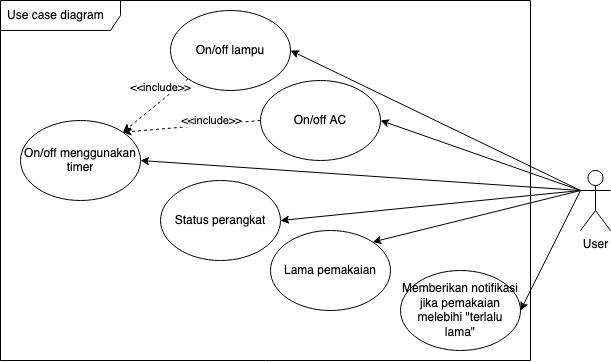
\includegraphics[scale=0.4]{diagrams/use-case.png}}
\caption{Diagram \textit{use case} sistem IoT yang dibuat}
\label{diag-use-case}
\end{figure}

Selain itu, ada sebuah aplikasi yang dapat digunakan untuk mengaktifkan
fitur-fitur terkait. Aplikasi ini akan digunakan oleh pengguna untuk
mengendalikan peralatan rumahnya dari jauh.

\subsection{Arsitektur Sistem}

\begin{figure}[htbp]
\centerline{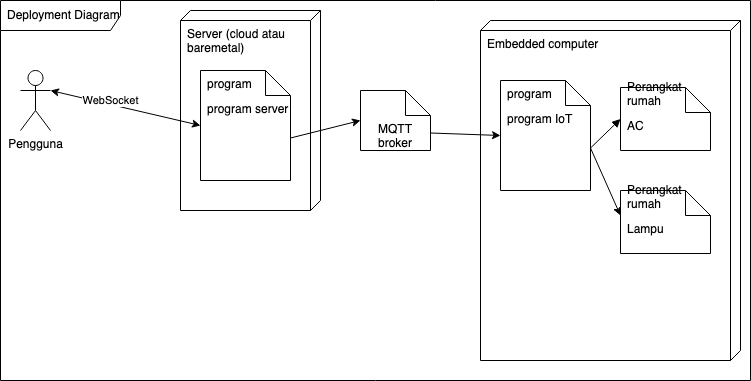
\includegraphics[scale=0.3]{diagrams/deployment-diagram.png}}
\caption{Diagram arsitektur sistem IoT yang dibuat}
\label{diag-deploy-diag}
\end{figure}

Melihat kebutuhan sistem, dibuat sistem yang memanfaatkan sebuah server.
Pada sistem yang dibuat, perangkat \textit{embedded computer} bertugas
sebagai antarmuka ke perangkat yang mematikan dan menyalakan lampu.
Sedangkan perintah mematikan dan menyalakan akan dikirimkan dari server
melalui MQTT. Server juga bertugas untuk mengendalikan \textit{timer}.
Jadi, aplikasi tidak akan langsung berkomunikasi dengan \textit{embbedded
computer}, akan tetapi aplikasi akan berkomunikasi dengan server terlebih
dahulu.

Lalu, aplikasi pengguna akan berupa \textit{web application} untuk
memudahkan pengembangan. Aplikasi pengguna dan server akan berkomunikasi
menggunakan WebSocket.

Arsitektur dapat dilihat dilihat pada gambar \ref{diag-deploy-diag}.

\section{Hasil Implementasi}\label{sect-hasil}
Semua fitur, kecuali fitur mematikan lampu dengan \textit{timer}, berhasil
diimplementasi. Akan tetapi ada beberapa kekurangan seperti fitur
\textit{timer} yang tidak menggunakan waktu perangkat dimatikan atau
dinyalakan, melainkan berapa detik hingga perangkat dinyalakan. Selain
itu, harus dilakukan \textit{refresh} secara manual jika status perangkat
diubah dari \textit{instance} aplikasi lain.

\begin{figure}[htbp]
\centerline{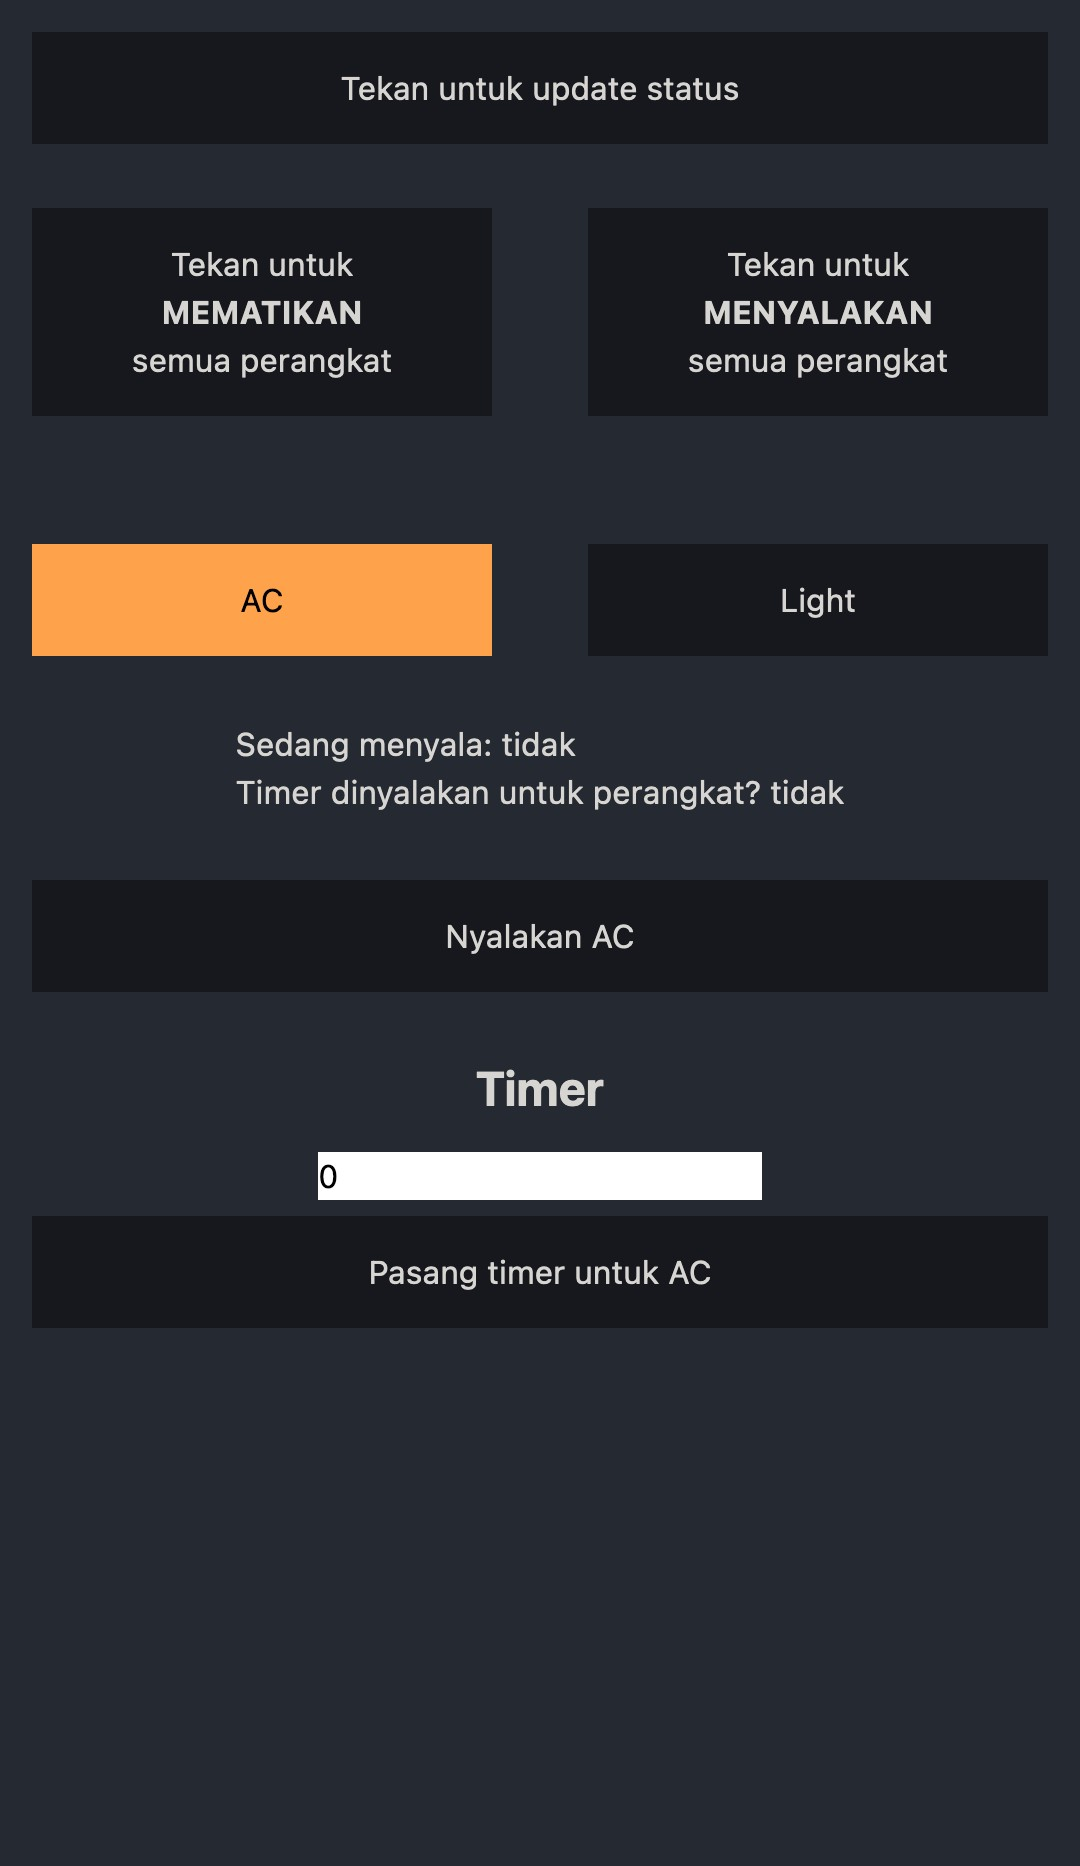
\includegraphics[scale=0.2]{other-images/messageImage_1679385387006.jpg}}
\caption{Diagram \textit{use case} sistem IoT yang dibuat}
\label{img-interface}
\end{figure}

Antarmuka aplikasi dapat dilihat pada gambar \ref{img-interface}.

Kode sumber aplikasi dan video demo dapat diakses pada Lampiran.

\section{Kesimpulan}\label{sect-kesimpulan}

\section*{Lampiran}

\begin{itemize}
    \item Kode sumber: \url{https://github.com/jspmarc/IF4051-UTS}
    \item Video demo: \url{https://drive.google.com/file/d/1YPXsKIWPC0QWv77nntUNKCLq5-i4OdfC/view?usp=share_link}
\end{itemize}

\end{document}
